\chapter{Data Analysis}
This project will investigate if there exists a cointegrating relation between the four cryptocurrencies namely, Bitcoin, Ethereum, Solana and Ripple. In this chapter, we will examine the data with visual interpretation of plots and qualitative tests.

\section{Data Introduction}
The data that has been used can be found at yahoo  [ref].\\
The data chosen for this project consists of opening prices, the daily lowest prices, the daily highest price and the closing prices all in USD for Bitcoin, Ethereum, Solana and Ripple. These have been chosen because of the amount of transaction volume and market capitalization, to evade coins that might be rug pulled and coins that are very explosive because of limited amount. The data from these Crypto currency's have been cleaned to only contain closing prices with no NA values. The data is then split into 2 with $90\%$ going towards the training data and the last $10\%$ as validation data. The training data is then used to make the model that can be foretasted. Finally the foretasted values can then be checked against the validation set to inspect the accuracy of our model. 
\newpage
\section{Leveled graph}
For the leveled graphs the closing prices will be plotted this will be done from Start-dato to slut-dato for all 4 Crypto currencies and can be found below, this is called the leveled graph.

\begin{figure}[h]
  \centering
  \subfloat[][]{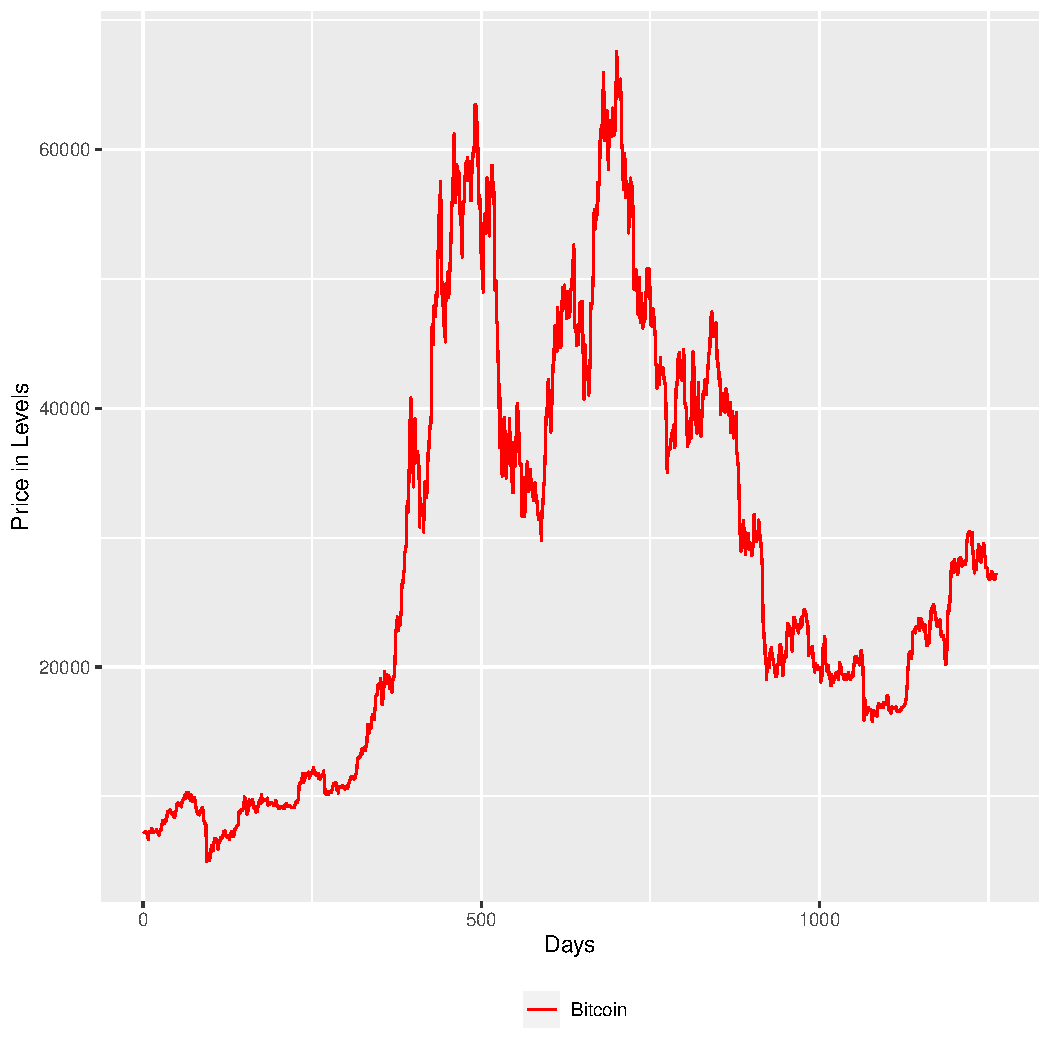
\includegraphics[width=.4\textwidth]{1.Projekt_kode/Billeder/Crypto_in_levels_Bitcoin.pdf}}\quad
  \subfloat[][]{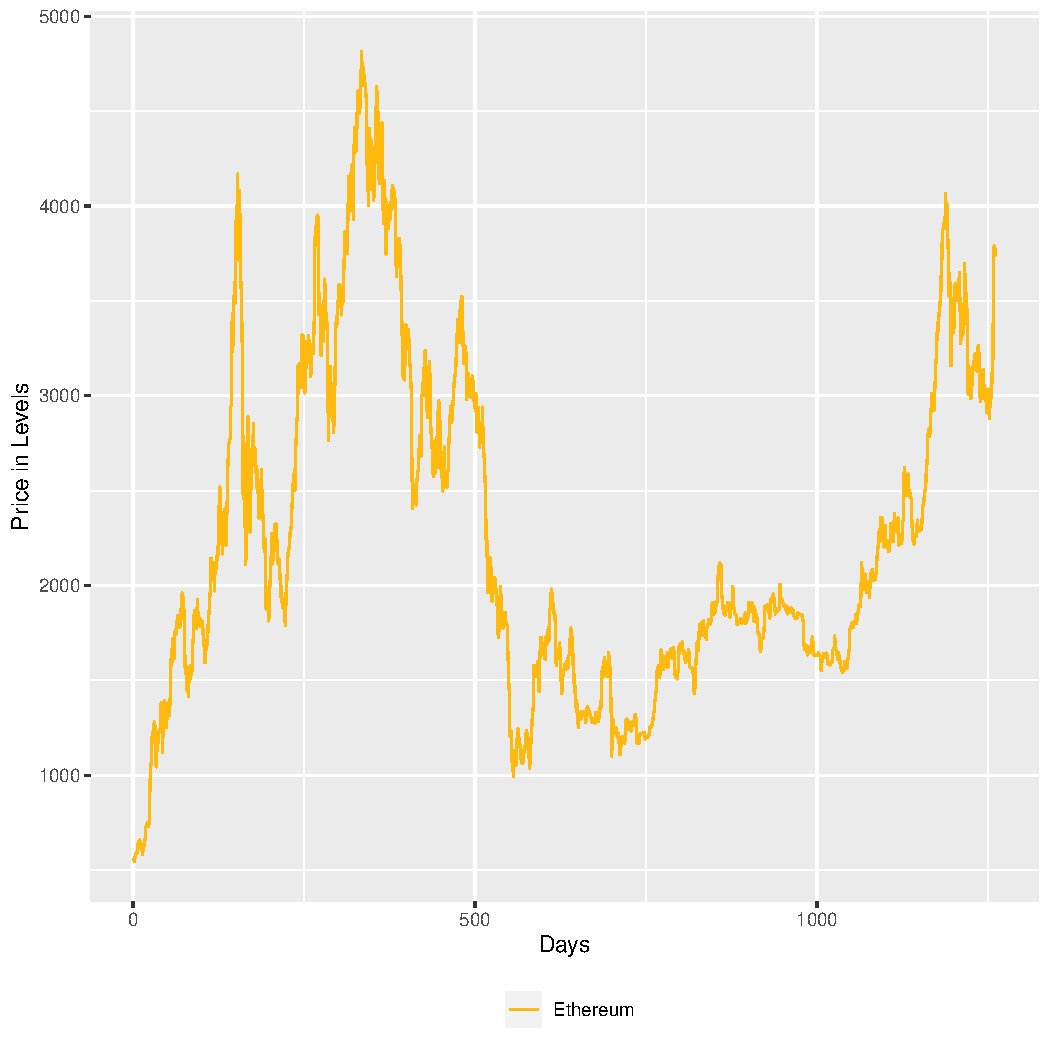
\includegraphics[width=.4\textwidth]{1.Projekt_kode/Billeder/Crypto_in_levels_Ethereum.pdf}}\\
  \subfloat[][]{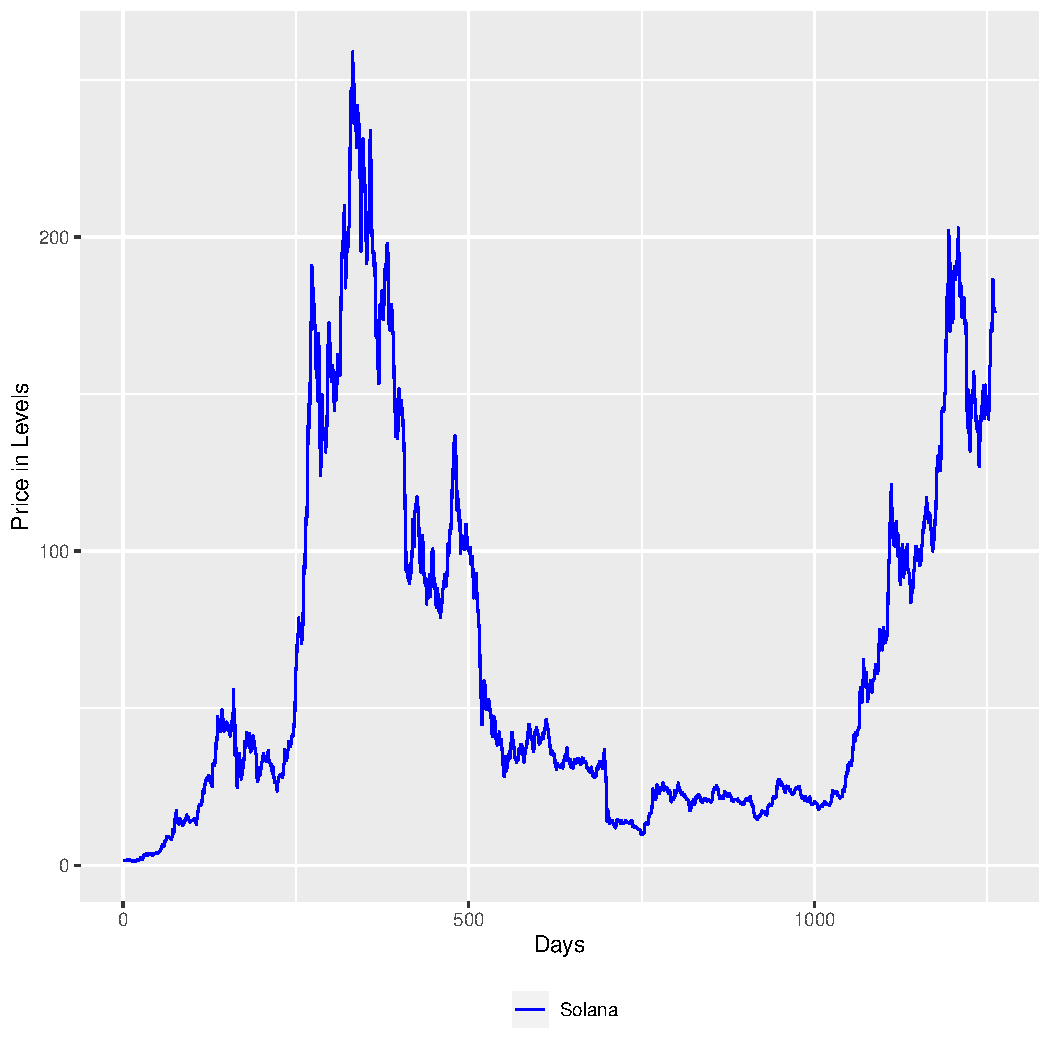
\includegraphics[width=.4\textwidth]{1.Projekt_kode/Billeder/Crypto_in_levels_Solana.pdf}}\quad
  \subfloat[][]{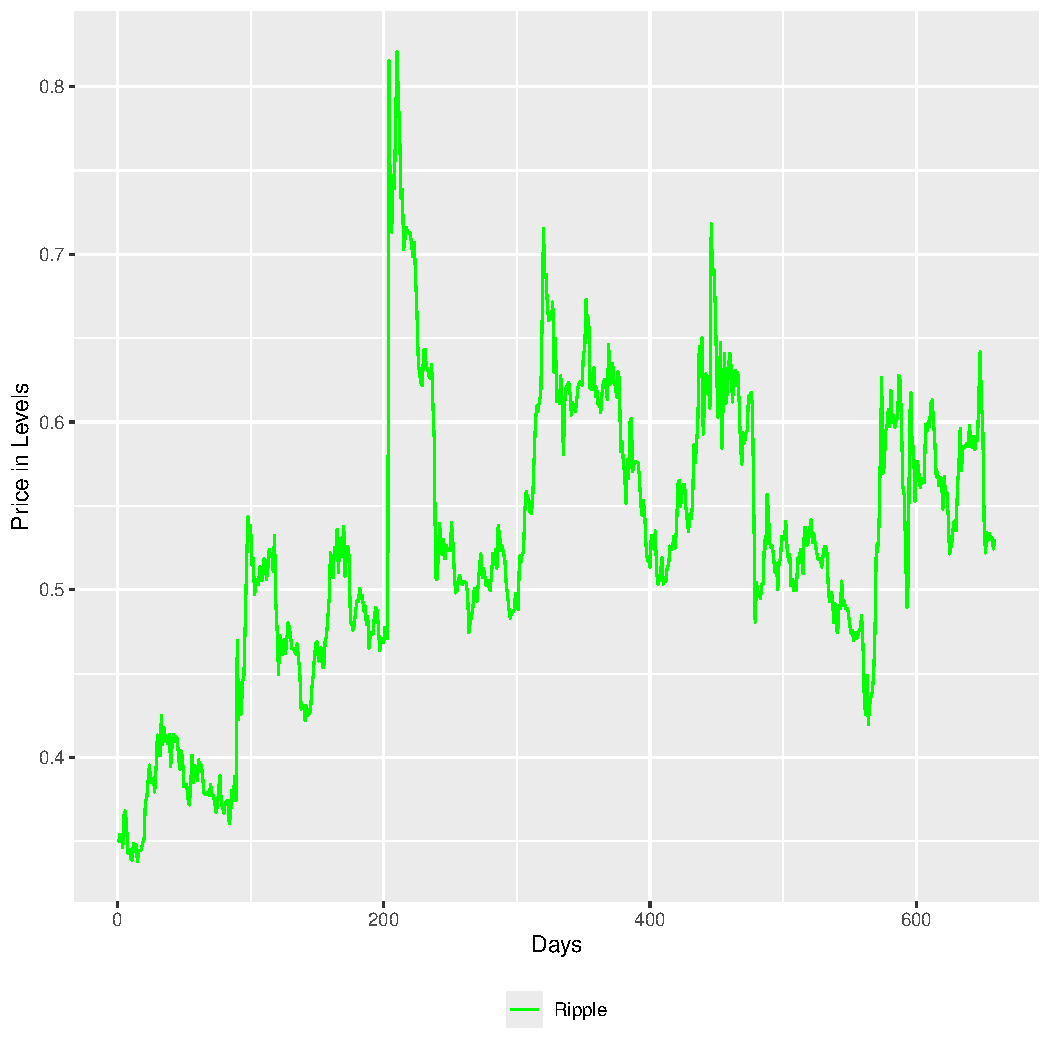
\includegraphics[width=.4\textwidth]{1.Projekt_kode/Billeder/Crypto_in_levels_Ripple.pdf}}
  \caption{First group of subfigures.}
  \label{graph_in _levels}
\end{figure}
\noindent looking at the 4 crypto currencies there are multiple similarity's for \ref{graph_in _levels} an example of this is that a,b and c all have a rise time $1000$ and forward of our training set and all four also have a somewhat low period in the middle of the data set, other similarity's can be found but we will not go into detail about all these instead the similarity's give an occasion to look at whether cointegration is possible which can be cheeked using the Johanson, and or Engle granger. Before this can be done, other tests must be made to check whether the data even can be cointegrated this is done checking for multiple things 
\begin{enumerate}
    \item Determining the number of lags
    \item check it is $I(1)$ and that the differenced data is stationary 
    \item Looking at QQ-plots
\end{enumerate}

\section{Model Validation}
Before examining whether cointegration is present it is nescessary to have the optimal amount of lags in our $VAR$ model which is done using the function $VARselect$ which provides four different tests; the AIC, HQ, BIC and FPE. Here the AIC is chosen since the AIC and BIC is preferred when forecasting. There are incentives for choosing both an AIC or BIC, the BIC is sometimes preferred for large sample sizes which is the case in this instance but in hindsight the BIC generally chooses a less complicated model since it penalizes extra parameters more than the AIC. This in unison with the fact that the BIC is often advantageous when the true model is present which we can not assume leads us to believe the AIC is more efficient since the price of cryptovalutas is also influenced by external factors not included in the model \cite{AICorBIC}.

\subsection{Check $I(1)$}
For the data to be cointegrating it  must be non-stationary of order 1 or $I(1)$ this is checked by differencing the data doing so takes $x_t-x_{t-1}$ and gives us the diffrenced data set the is then used to plot these 3 graphs that is seen here. The first in the top left of the 4 pictures is the Histogram and checks that the data is noormally distributed so no constant is present. The second is the top right ACF function plot to check for quick decay and that no seasonality is present and looking at the plots there does not seam to be a indication that there is slow decay or seasonality so the conclusion must be that the data is stationary which is further backed up by the last picture the graph of the diffed values, that is stationary around zero. this is true for all 4 time series seen in the graphs below
\begin{figure}[H]
  \centering
  \subfloat[][]{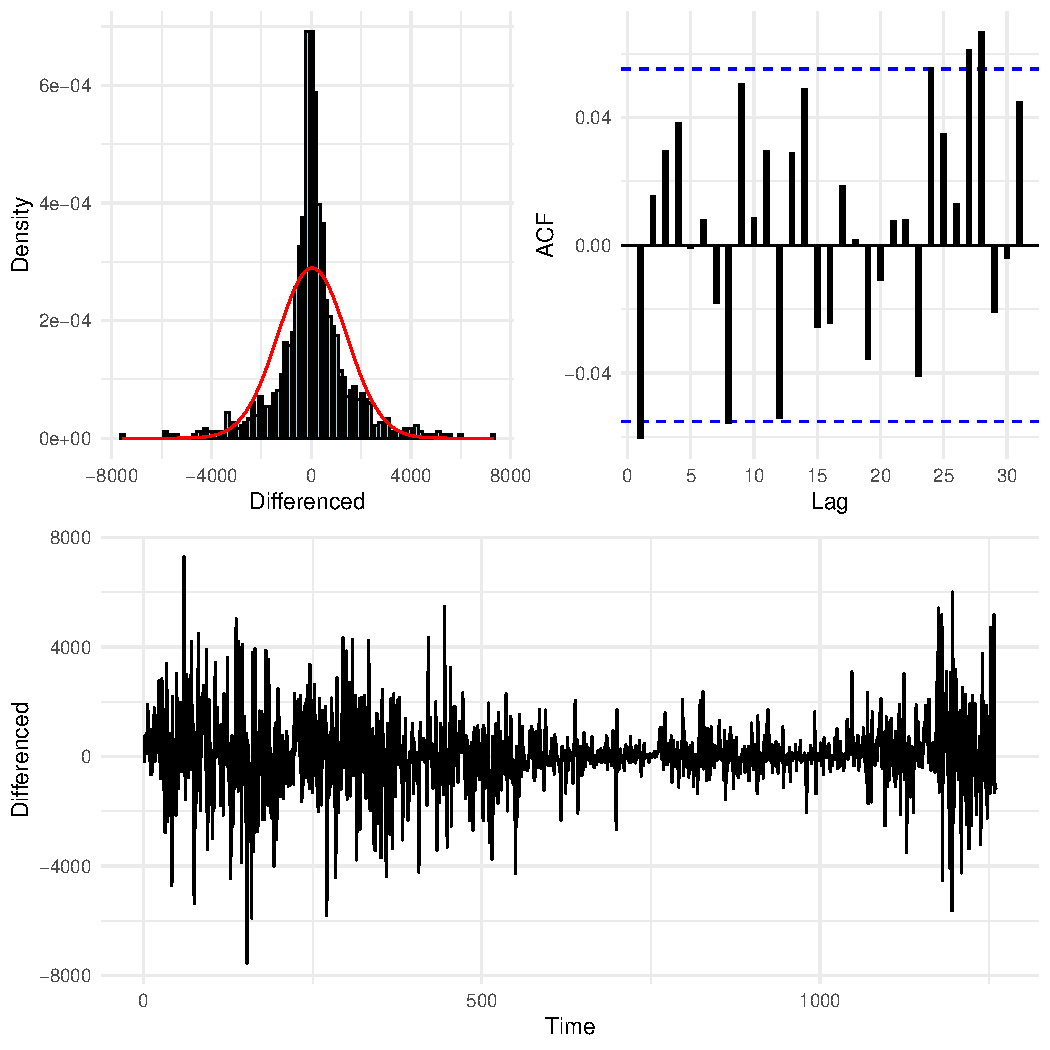
\includegraphics[width=.4\textwidth]{1.Projekt_kode/Billeder/plot_grid_Bitcoin.pdf}}\quad
  \subfloat[][]{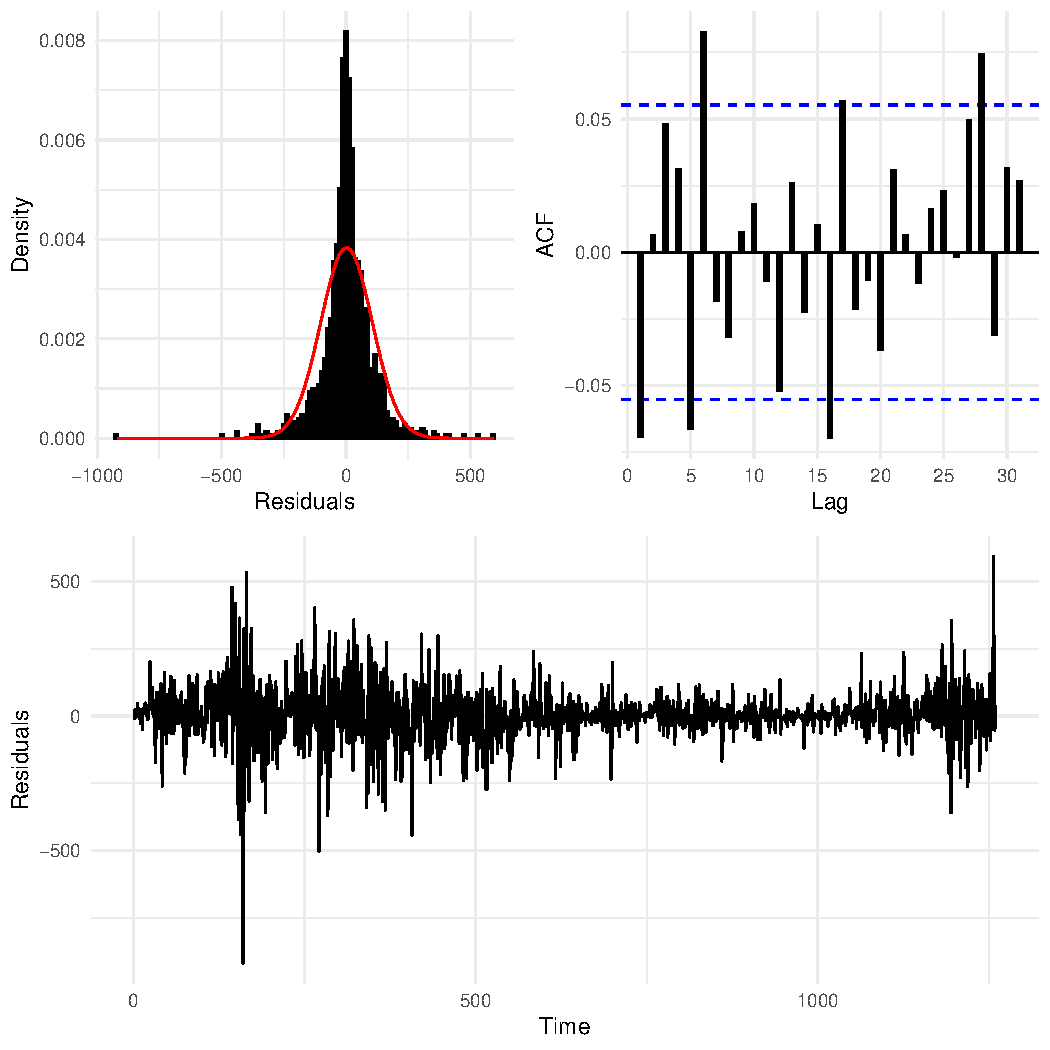
\includegraphics[width=.4\textwidth]{1.Projekt_kode/Billeder/plot_grid_Ethereum.pdf}}\\
  \subfloat[][]{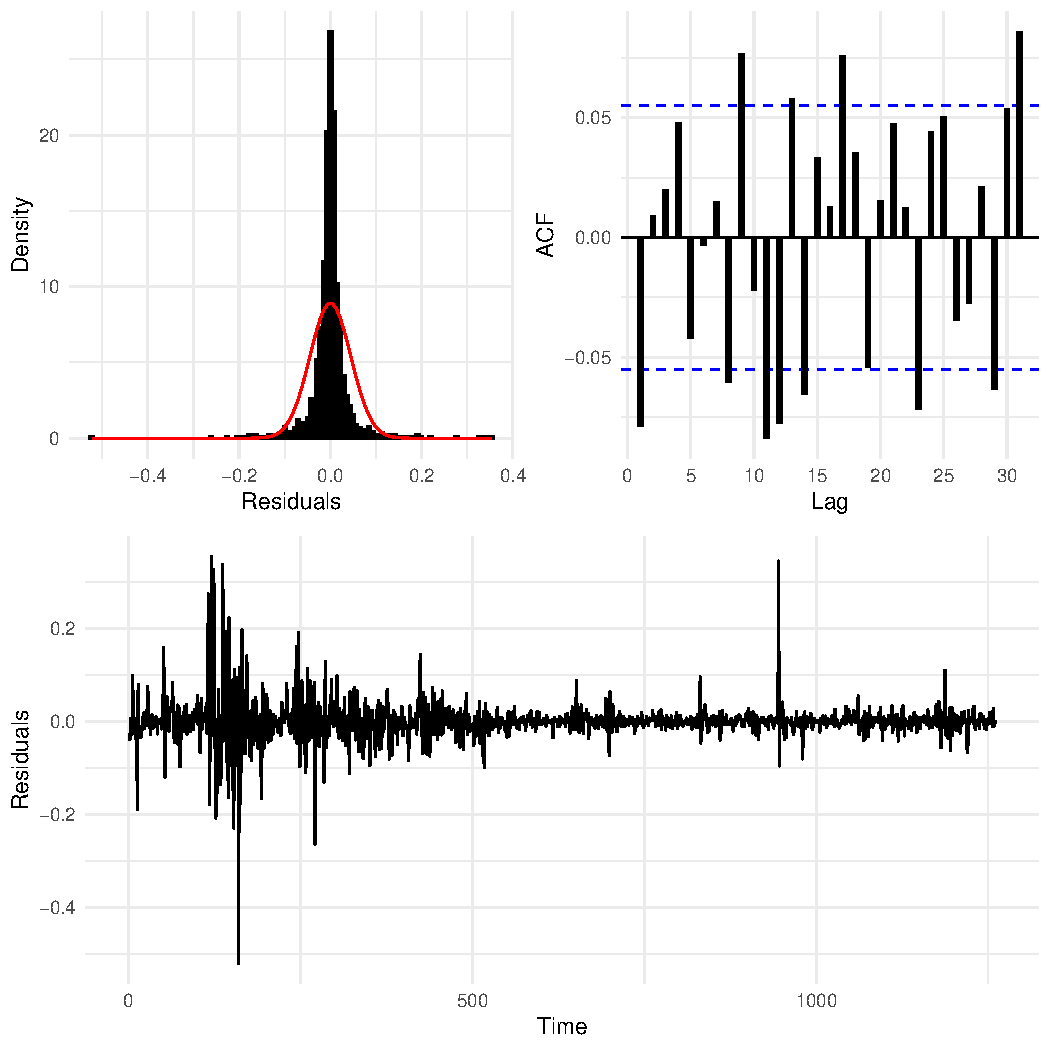
\includegraphics[width=.4\textwidth]{1.Projekt_kode/Billeder/plot_grid_Ripple.pdf}}\quad
  \subfloat[][]{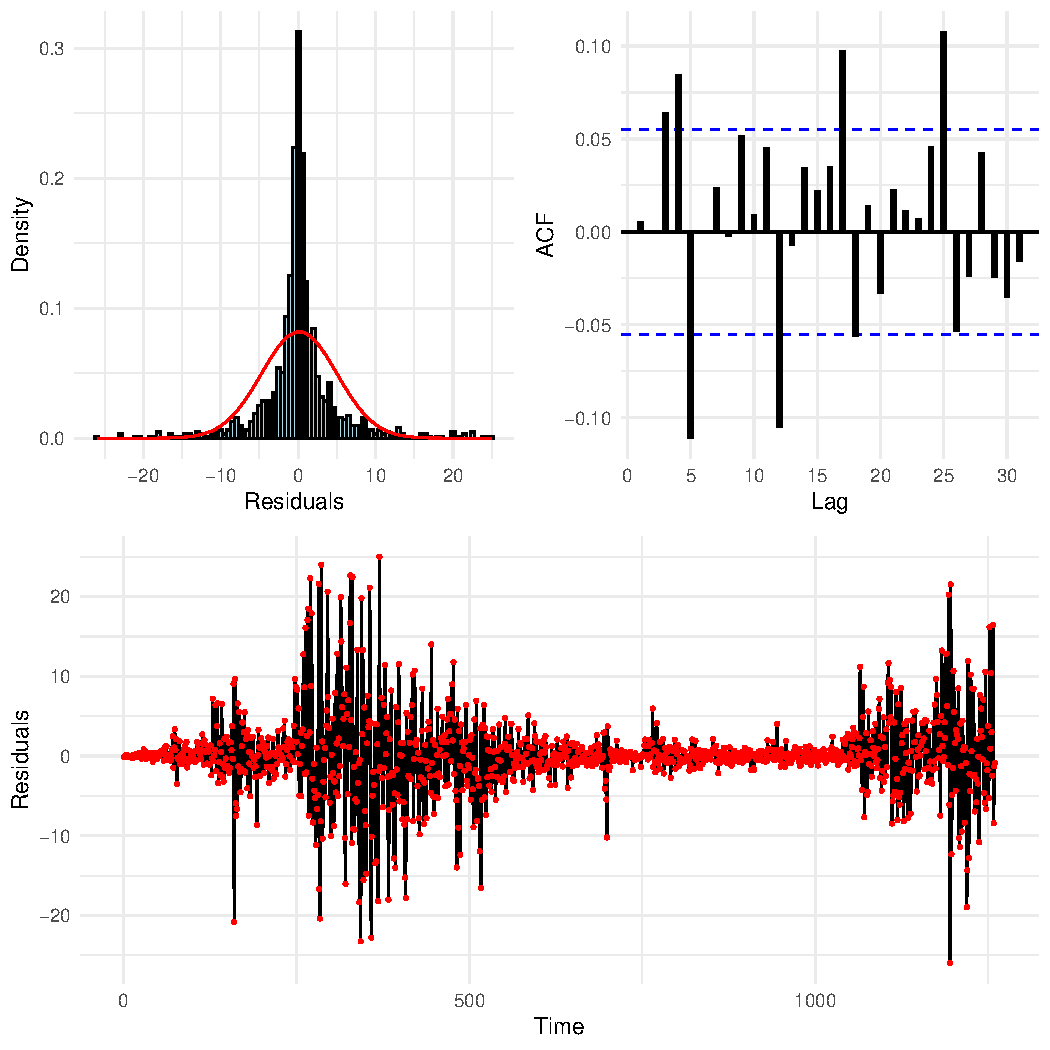
\includegraphics[width=.4\textwidth]{1.Projekt_kode/Billeder/plot_grid_Solana.pdf}}
  \caption{(a) Bitcoin, (b) Ethereum, (c) Ripple, (d) Solana }
\end{figure}
\newpage
\subsection{QQ-plots}

Looking at the quintile quintile plots also called QQ-plots it must be checked that the data is normally distributed and valued if there is an existence of heavy tails.
\begin{figure}[H]
  \centering
  \subfloat[][]{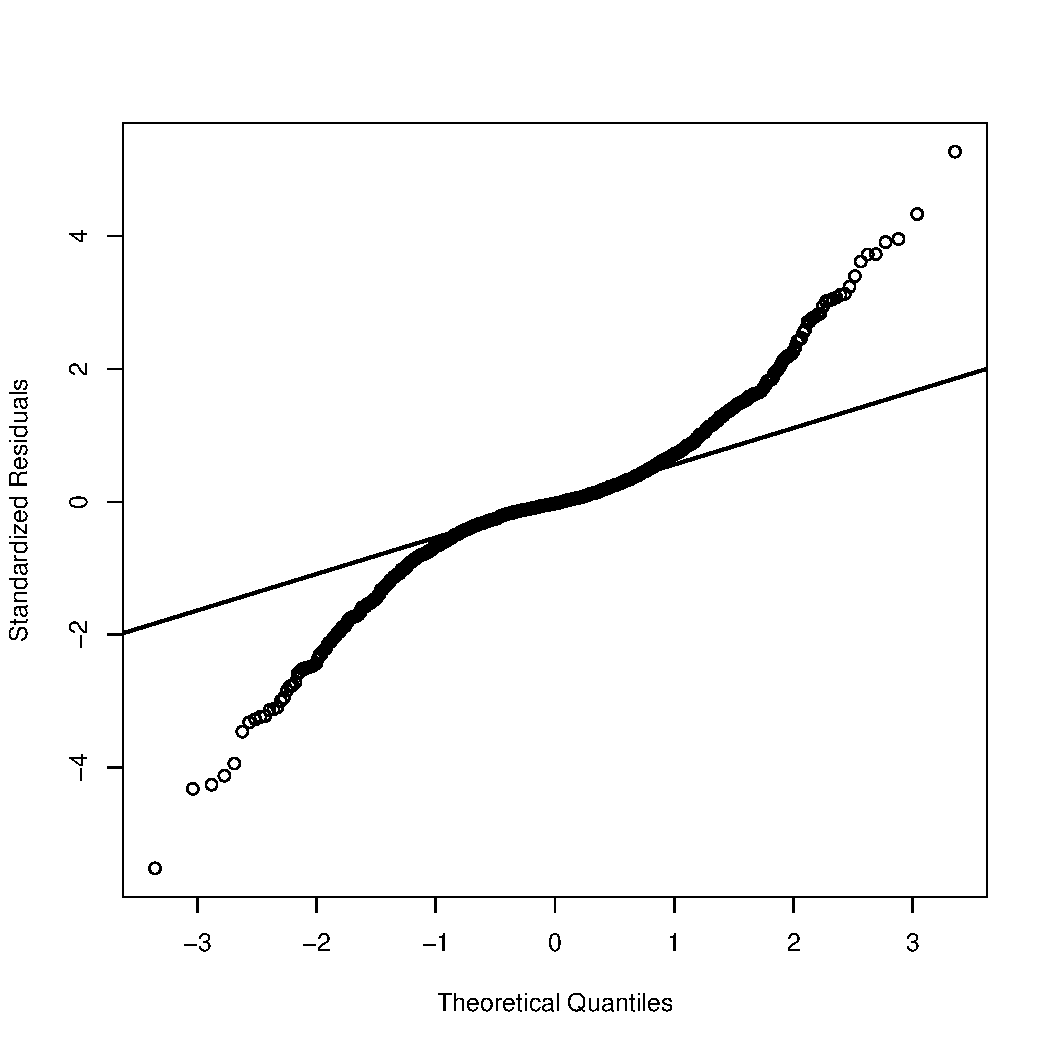
\includegraphics[width=.35\textwidth]{1.Projekt_kode/Billeder/qqplot_Bitcoin.pdf}}\quad
  \subfloat[][]{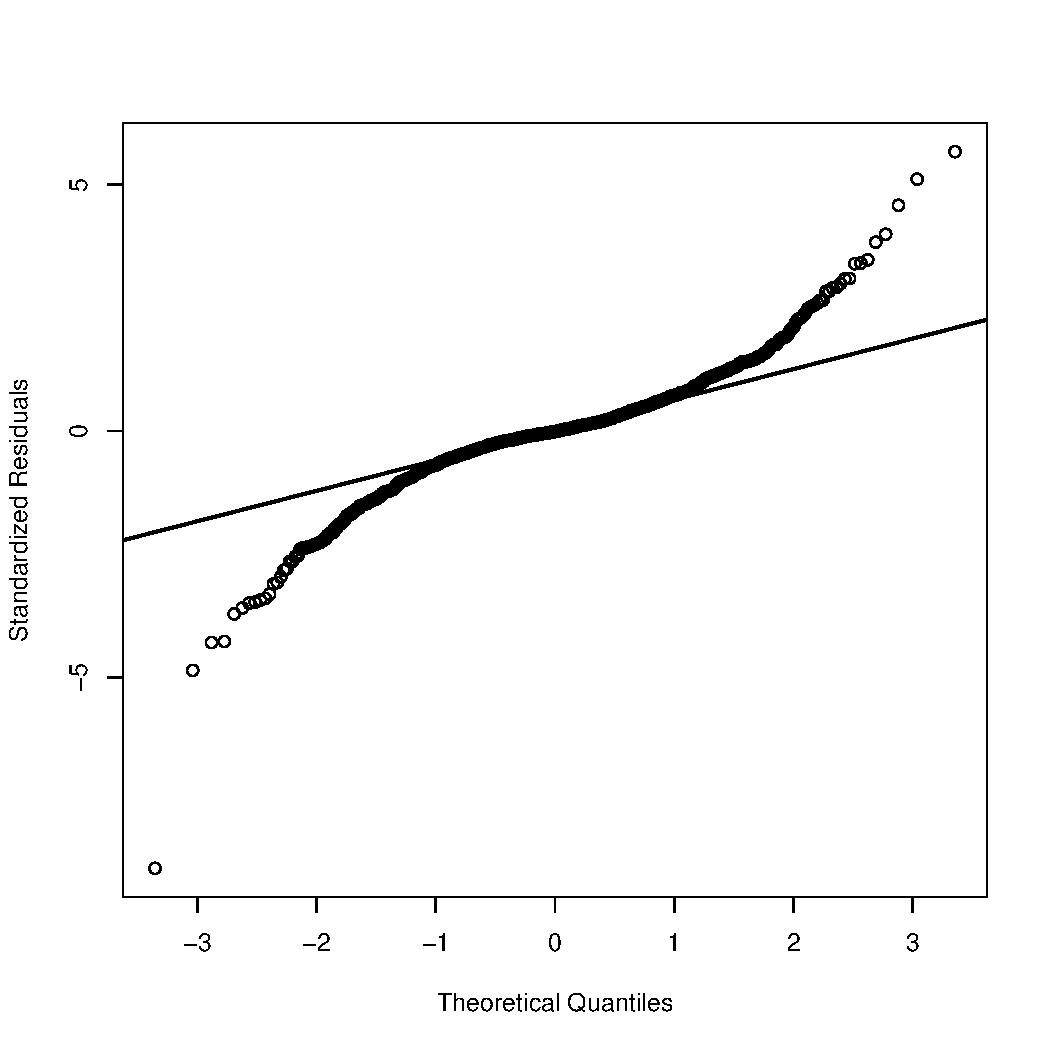
\includegraphics[width=.35\textwidth]{1.Projekt_kode/Billeder/qqplot_Ethereum.pdf}}\\
  \subfloat[][]{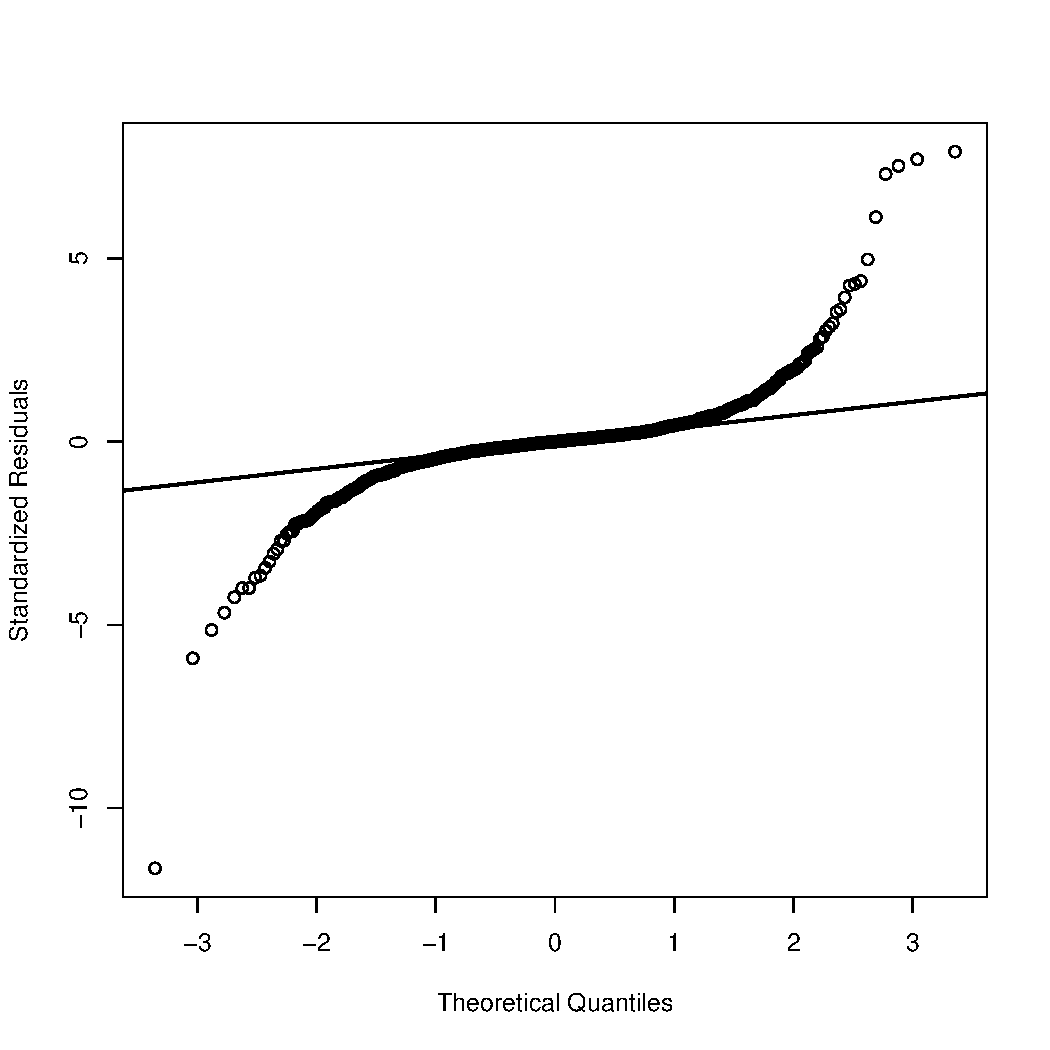
\includegraphics[width=.35\textwidth]{1.Projekt_kode/Billeder/qqplot_Ripple.pdf}}\quad
  \subfloat[][]{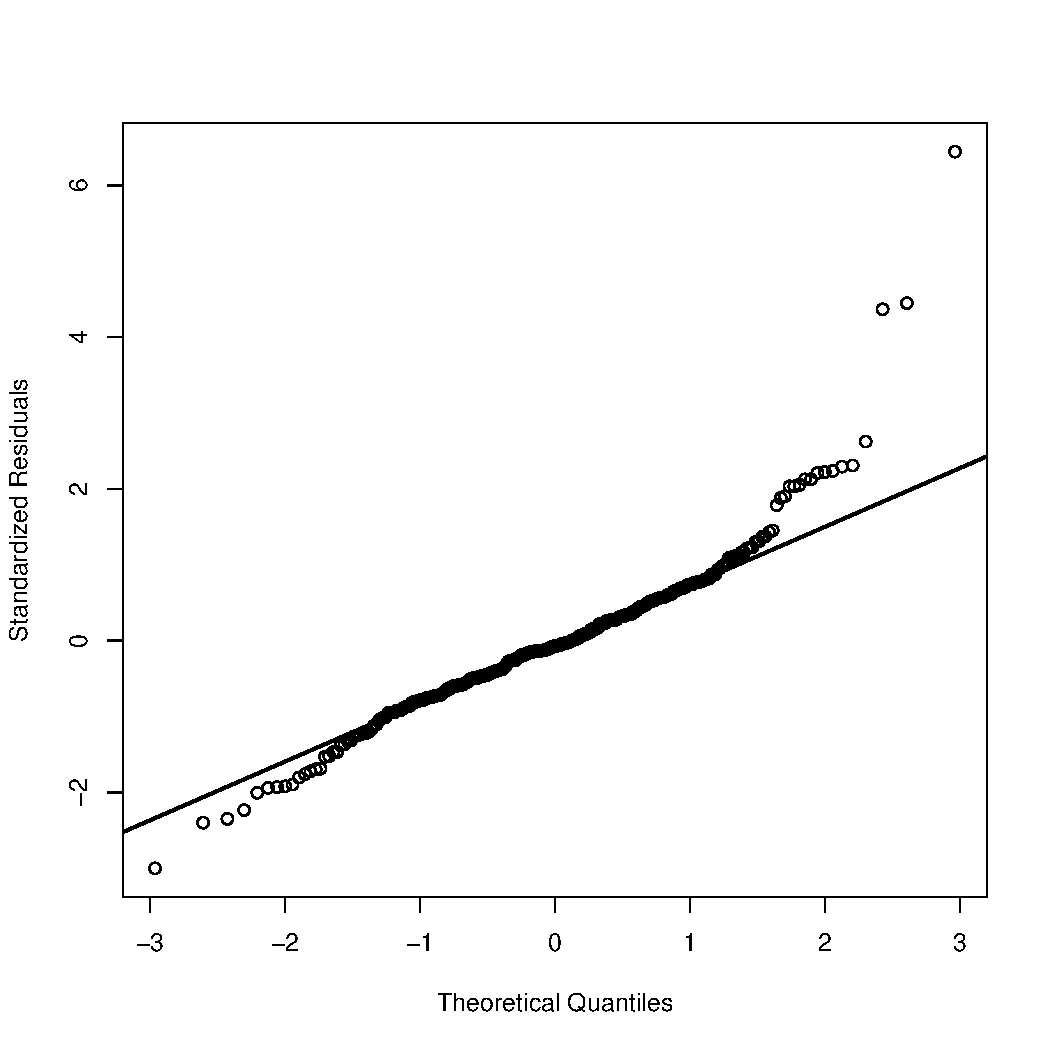
\includegraphics[width=.35\textwidth]{1.Projekt_kode/Billeder/qqplot_Solana.pdf}}
  \caption{(a) Bitcoin, (b) Ethereum, (c) Ripple, (d) Solana }
\end{figure}
Looking at the QQ-plots it clear to see that all the differenced data is symmetric in their respective QQ-plots but all have heavy tails meaning that they have more extreme values than a normal distribution, this can also be seen earlier in the histogram. This is something to consider when evaluating the model, but for now the data is still considered normally distributed.